% EMSE version: Springer Nature LaTeX template (sn-jnl.cls 3.1) with name-year references (sn-basic), as EMSE asks.
% The AUSE version is main.tex; both share refs.bib and generated/.
\documentclass[pdflatex,sn-basic]{sn-jnl}
\usepackage[T1]{fontenc}
\usepackage{microtype}
\usepackage{graphicx}
\usepackage{booktabs}
\usepackage{tabularx}
\usepackage{array}
\usepackage{amsmath}
\usepackage{xcolor}
\usepackage[title]{appendix}

\newcommand{\NClaudeRuns}{792}
\newcommand{\NClaudeSessions}{899}
\newcommand{\NLocalRuns}{48}
\newcommand{\NAllRuns}{840}
\newcommand{\NAllSessions}{975}
\newcommand{\NVerifyOk}{773}
\newcommand{\NVerifyHaikuFail}{15}
\newcommand{\NVerifyFail}{19}
\newcommand{\TotalCost}{\$64}
\newcommand{\PoolMissCost}{$-$14\%}
\newcommand{\PoolMissCI}{$-$22\% to $-$5\%}
\newcommand{\PoolMissProse}{17/56}
\newcommand{\PoolMissRules}{0/56}
\newcommand{\PoolLoadedCost}{0\%}
\newcommand{\PoolLoadedCI}{$-$11\% to +12\%}
\newcommand{\PoolLoadedProse}{0/32}
\newcommand{\PoolLoadedRules}{0/32}
\newcommand{\HThreeNoLoop}{47/48}
\newcommand{\HThreeNoLoopCI}{89\% to 100\%}
\newcommand{\HThreeNoPointer}{48/48}
\newcommand{\HThreeNoPointerCI}{93\% to 100\%}
\newcommand{\HThreeFull}{47/48}
\newcommand{\HThreeFullCI}{89\% to 100\%}
\newcommand{\HOneBreaks}{8/48}
\newcommand{\HOneBreaksAgainst}{0/48}
\newcommand{\HOneBreaksP}{0.001}
\newcommand{\HOneCost}{+12\%}
\newcommand{\HOneCI}{0\% to +24\%}
\newcommand{\HOneCostP}{0.024}
\newcommand{\HOneN}{96}
\newcommand{\HTwoBreaks}{0/48}
\newcommand{\HTwoBreaksAgainst}{0/48}
\newcommand{\HTwoBreaksP}{1.000}
\newcommand{\HTwoCost}{+13\%}
\newcommand{\HTwoCI}{+3\% to +24\%}
\newcommand{\HTwoCostP}{0.005}
\newcommand{\HTwoN}{96}
\newcommand{\HFourBreaks}{0/5}
\newcommand{\HFourBreaksAgainst}{0/5}
\newcommand{\HFourBreaksP}{1.000}
\newcommand{\HFourCost}{+9\%}
\newcommand{\HFourCI}{$-$9\% to +30\%}
\newcommand{\HFourCostP}{0.177}
\newcommand{\HFourN}{10}
\newcommand{\HFiveBreaks}{3/16}
\newcommand{\HFiveBreaksAgainst}{0/16}
\newcommand{\HFiveBreaksP}{0.100}
\newcommand{\HFiveCost}{+20\%}
\newcommand{\HFiveCI}{+1\% to +42\%}
\newcommand{\HFiveCostP}{0.016}
\newcommand{\HFiveN}{32}
\newcommand{\HSevenBreaks}{3/32}
\newcommand{\HSevenBreaksAgainst}{0/32}
\newcommand{\HSevenBreaksP}{0.121}
\newcommand{\HSevenCost}{+1\%}
\newcommand{\HSevenCI}{$-$9\% to +13\%}
\newcommand{\HSevenCostP}{0.428}
\newcommand{\HSevenN}{64}
\newcommand{\HNineBreaks}{4/32}
\newcommand{\HNineBreaksAgainst}{0/32}
\newcommand{\HNineBreaksP}{0.056}
\newcommand{\HNineCost}{$-$3\%}
\newcommand{\HNineCI}{$-$12\% to +8\%}
\newcommand{\HNineCostP}{0.691}
\newcommand{\HNineN}{64}
\newcommand{\HElevenBreaks}{0/64}
\newcommand{\HElevenBreaksAgainst}{0/64}
\newcommand{\HElevenBreaksP}{1.000}
\newcommand{\HElevenCost}{+3\%}
\newcommand{\HElevenCI}{$-$19\% to +29\%}
\newcommand{\HElevenCostP}{0.402}
\newcommand{\HElevenN}{128}
\newcommand{\HSixBreaks}{3/16}
\newcommand{\HSixBreaksAgainst}{0/16}
\newcommand{\HSixBreaksP}{0.100}
\newcommand{\HSixCost}{+20\%}
\newcommand{\HSixCI}{+1\% to +42\%}
\newcommand{\HSixCostP}{0.016}
\newcommand{\HSixN}{32}
\newcommand{\HEightBreaks}{3/32}
\newcommand{\HEightBreaksAgainst}{0/32}
\newcommand{\HEightBreaksP}{0.121}
\newcommand{\HEightCost}{+1\%}
\newcommand{\HEightCI}{$-$9\% to +13\%}
\newcommand{\HEightCostP}{0.428}
\newcommand{\HEightN}{64}
\newcommand{\HTenBreaks}{4/32}
\newcommand{\HTenBreaksAgainst}{0/32}
\newcommand{\HTenBreaksP}{0.056}
\newcommand{\HTenCost}{$-$3\%}
\newcommand{\HTenCI}{$-$12\% to +8\%}
\newcommand{\HTenCostP}{0.691}
\newcommand{\HTenN}{64}
\newcommand{\SeqOk}{16}
\newcommand{\SeqPlanned}{48}
\newcommand{\HOneCatchFull}{45}
\newcommand{\HTwoCatchNoPointer}{115}
\newcommand{\PoolFourFiveBreaks}{7/64}
\newcommand{\PoolFourFiveP}{0.007}
\newcommand{\NoneVsProseCost}{+35\%}
\newcommand{\NoneVsProseCI}{+21\% to +50\%}
\newcommand{\TaxCost}{+9\%}
\newcommand{\TaxCI}{$-$7\% to +27\%}
\newcommand{\GenBreaks}{0/48}
\newcommand{\GenCost}{$-$25\%}
\newcommand{\GenCI}{$-$32\% to $-$17\%}
\newcommand{\NLoopRuns}{360}
\newcommand{\NLoopBroken}{0}
\newcommand{\PSixPrimaryRuns}{256}
\newcommand{\PSixLocalRuns}{128}
\newcommand{\PSixLatestRuns}{56}
\newcommand{\PSixRuns}{440}
\newcommand{\NTotalRuns}{1280}
\newcommand{\NTotalSessions}{1532}
\newcommand{\PSixCost}{\$163}
\newcommand{\NTotalCost}{\$227}
\newcommand{\HTwelveProse}{28/128}
\newcommand{\HTwelveRules}{17/128}
\newcommand{\HTwelveP}{0.048}
\newcommand{\HTwelveHolm}{0.095}
\newcommand{\HThirteenCost}{+6\%}
\newcommand{\HThirteenCI}{$-$5\% to +18\%}
\newcommand{\HThirteenP}{0.281}
\newcommand{\HThirteenHolm}{0.281}
\newcommand{\HThirteenTaskCost}{+9\%}
\newcommand{\HThirteenTaskCI}{$-$2\% to +21\%}
\newcommand{\PSixBPProse}{15/64}
\newcommand{\PSixBPRules}{16/64}
\newcommand{\PSixBPP}{0.659}
\newcommand{\PSixFBProse}{13/64}
\newcommand{\PSixFBRules}{1/64}
\newcommand{\PSixFBP}{$<$0.001}
\newcommand{\HFourteenProse}{47/64}
\newcommand{\HFourteenRules}{19/64}
\newcommand{\HFourteenP}{$<$0.001}
\newcommand{\PSixBPCatchRuns}{38/64}
\newcommand{\PSixBPIgnoredRuns}{16}
\newcommand{\PSixBPRoleRuns}{31/31}
\newcommand{\PSixBPRoleTFour}{31/31}
\newcommand{\PSixOpened}{32/64}
\newcommand{\PSixOpenedViol}{4/32}
\newcommand{\PSixNotOpenedViol}{6/32}
\newcommand{\PSixBPCells}{1482}
\newcommand{\PSixBPPrecision}{6/16}
\newcommand{\PSixBPPrecisionCI}{15\% to 65\%}
\newcommand{\PSixBPRecall}{6/28}
\newcommand{\PSixBPRecallCI}{8\% to 41\%}
\newcommand{\PSixFBCells}{120}
\newcommand{\PSixFBPrecision}{13/13}
\newcommand{\PSixFBPrecisionCI}{75\% to 100\%}
\newcommand{\PSixFBRecall}{13/13}
\newcommand{\PSixFBRecallCI}{75\% to 100\%}
\newcommand{\PSixBPFpRole}{10}
\newcommand{\PSixBPFnNoAny}{13}
\newcommand{\PSixBPFnZod}{6}
\newcommand{\PSixBPFnOther}{3}
\newcommand{\PSixLoopFalse}{6/82}
\newcommand{\PSixLoopFalseCI}{3\% to 15\%}
\newcommand{\PSixAfterFalse}{2/170}
\newcommand{\PSixAfterFalseCI}{0\% to 4\%}
\newcommand{\PSixBPConventions}{40}
\newcommand{\PSixBPLOC}{491}
\newcommand{\PSixBPCases}{91}
\newcommand{\PSixFBConventions}{4}
\newcommand{\PSixFBLOC}{151}
\newcommand{\PSixFBCases}{18}
\newcommand{\PSevenRuns}{128}
\newcommand{\NTotalRunsEMSE}{1408}
\newcommand{\NTotalSessionsEMSE}{1691}
\newcommand{\PSevenCost}{\$22}
\newcommand{\HSixteenProse}{31/64}
\newcommand{\HSixteenRules}{0/64}
\newcommand{\HSixteenP}{$<$0.001}
\newcommand{\HSixteenHolm}{$<$0.001}
\newcommand{\HSeventeenCost}{$-$24\%}
\newcommand{\HSeventeenCI}{$-$30\% to $-$18\%}
\newcommand{\HSeventeenP}{1.000}
\newcommand{\HSeventeenHolm}{1.000}
\newcommand{\HSeventeenTaskCost}{$-$1\%}
\newcommand{\HSeventeenTaskCI}{$-$8\% to +7\%}
\newcommand{\PSevenDOneProse}{29/64}
\newcommand{\PSevenDOneP}{$<$0.001}
\newcommand{\PSevenAsCast}{21}
\newcommand{\PSevenManager}{7}
\newcommand{\PSevenHelpers}{1}
\newcommand{\PSevenLoopRuns}{38}
\newcommand{\PSevenIgnoredRuns}{0}
\newcommand{\PSevenProseLeft}{1}
\newcommand{\PSevenTurnsProse}{31.7}
\newcommand{\PSevenTurnsRules}{25.5}
\newcommand{\PSevenVerifyProse}{58/64}
\newcommand{\PSevenVerifyProseCI}{81\% to 96\%}
\newcommand{\PSevenVerifyProseFail}{6}
\newcommand{\PSevenVerifyProseTTwo}{4}
\newcommand{\PSevenVerifyRules}{54/64}
\newcommand{\PSevenVerifyRulesCI}{73\% to 92\%}
\newcommand{\PSevenVerifyRulesFail}{10}
\newcommand{\PSevenVerifyRulesTTwo}{10}

% \input is not expandable inside a tabular, so a rule after it fails; the primitive is.
\makeatletter\let\rows\@@input\makeatother
\emergencystretch=3em
\raggedbottom

\newcommand{\file}[1]{\texttt{#1}}
\newcommand{\arm}[1]{\texttt{#1}}
\newcolumntype{L}{>{\raggedright\arraybackslash}X}

% ORCID link as text: the class expects Orcidlogo.eps, which the upload does not need.
\renewcommand{\orcidlogo}{\textsuperscript{\,ORCID}}
\begin{document}

\title[Where Should a Coding Rule Live?]{Where Should a Coding Rule Live? A Controlled Benchmark of Prose Instructions and Lint Rules for AI Coding Agents}

\author*{\fnm{Clirim} \sur{Ajeti}\orcid{https://orcid.org/0009-0000-7976-2785}}\email{clirimajeti@gmail.com}
\affil*{\orgname{Independent Researcher}, \orgaddress{\city{Munich}, \country{Germany}}}

\abstract{\textbf{Context.}
Teams write conventions for AI coding agents in Markdown instruction files such as \file{CLAUDE.md} and \file{AGENTS.md}, but nothing enforces them.
An alternative is a lint rule that runs after every edit and reports violations to the agent.

\textbf{Objective.}
We ask where a coding rule should live to minimize violations and cost.

\textbf{Method.}
We present agent-rules-bench, an open-source harness that runs the same task in identical repository copies, one per rule placement, and measures violations, cost and functional correctness.
We report \NTotalRuns{} agent runs on four projects in three languages: four exploratory studies and six pre-registered ones, the last registered on OSF.

\textbf{Results.}
When the rule was in prose that the agent could miss, it was violated in 17 of 56 exploratory runs, and as a lint rule in none.
Pre-registered, the feedback loop prevented violations of a rule that no prose stated (\HOneBreaks{} vs.\ \HOneBreaksAgainst), a one-line pointer avoided rework, and a 15.7k-token always-loaded file cost 20\% more.
Against conventions in a short always-loaded file, lint rules gained nothing.
In the largest study, the pooled advantage of lint rules was not significant after correction (\HTwelveProse{} vs.\ \HTwelveRules{} violating runs); it came from the project whose prose the agent did not load (\PSixFBProse{} vs.\ \PSixFBRules) and from a local model (\HFourteenProse{} vs.\ \HFourteenRules).
Functional correctness did not differ.

\textbf{Conclusions.}
Lint rules with an in-session feedback loop help where the agent does not read the prose.
Teams can keep always-loaded prose short and move the rules that agents miss into lint rules.}

\keywords{AI coding agents, coding conventions, static analysis, lint rules, context files, pre-registration}

\maketitle


\section{Introduction}
\label{sec:intro}

Teams state their conventions in repository instruction files, which AI coding agents such as Claude Code, Codex and pi read.
Typical conventions are ``inject a clock instead of calling \texttt{now()}'', ``keep database access out of route handlers'', and ``return success messages only from the API layer''.
These files grow.
A rule can then sit in the middle of long text, or in a linked document that the agent does not open.
The agent then copies the nearby code, and the nearby code often violates the rule.
This is especially true for legacy code.

A second place for a rule is a lint rule.
A linter tool checks the code, not the agent's attention.
If a hook runs the linter after every edit, the agent gets the message while it works, and it can fix the violation in the same session.
Practitioners recommend this approach \citep{evilmartians2026hooks}, but we found no controlled data on it.
Research on agent context files measures whether the files help at all \citep{gloaguen2026agentsmd,khatri2026contextfiles}, how their structure changes adherence \citep{mcmillan2026adherence}, and what they contain \citep{chatlatanagulchai2025agentreadmes}.
It does not compare prose with lint rules for the same rule.

This paper asks one question:
\emph{where should a coding rule live so that an AI coding agent follows it, and what does each place cost?}
We compare five places: prose in a linked document, prose buried in long documents, prose in the always-loaded file, a lint rule with a feedback loop, and a lint rule with a feedback loop and a one-line pointer.

Our contributions are:
\begin{enumerate}
\item \textbf{agent-rules-bench}, an open harness that runs headless agent sessions against identical repository copies, one copy per setup, and measures rule violations on added lines, cost, turns, review-fix rounds and functional correctness (Section~\ref{sec:method}).
\item \textbf{\NTotalRuns{} runs} on four public projects in three languages, with all setups, prompts, transcripts, diffs and logs published.
\item \textbf{Six pre-registered study plans} that test the parts of the lint setup separately, the cost of always-loaded prose, and prose against lint rules on two projects with two model families (Section~\ref{sec:results}).
\item \textbf{Measurement checks} of the checkers and the feedback loop: hand labels of a blind sample of diffs, and of every finding that the loop reported (Section~\ref{sec:plan6}).
\item \textbf{A practical guideline} for teams that write agent instructions (Section~\ref{sec:discussion}).
\end{enumerate}

\section{Background and Related Work}
\label{sec:related}

\paragraph{Context files for coding agents.}
Claude Code loads \file{CLAUDE.md} from the repository root at session start, and loads \file{CLAUDE.md} files in subdirectories when it reads files there.
Codex and pi load \file{AGENTS.md}, and Cursor reads its own rule files.
Several studies analyze what developers write in these files.
\citet{chatlatanagulchai2025manifests} study 253 \file{CLAUDE.md} files and find mostly build commands, implementation details and architecture; \citet{chatlatanagulchai2025agentreadmes} extend this to 2,303 context files of three agents.
\citet{jiang2026cursorrules} build a taxonomy of the context that developers give in Cursor rules, from 401 repositories.
\citet{gloaguen2026agentsmd} find that context files do not generally improve task success, and that they raise inference cost by over 20\% on average.
They also report that agents follow the instructions in these files well, and that the files are useful to state non-standard coding practices.
\citet{khatri2026contextfiles} finds, in an ablation with Claude Code and Codex, that the context strategy does not measurably change correctness: the agents fail on implementation skill, not on missing repository knowledge.
\citet{mcmillan2026adherence} varies four structural properties of configuration files (size, instruction position, file architecture and conflicting files) in 1,650 Claude Code sessions, and finds no detectable effect of any of them on adherence.
The largest effect in that study is within the session: adherence tends to fall as the agent generates more code.
All of these studies treat the context file as the only place for instructions.
We add the lint rule as a second place and compare both places for the same rule.

\paragraph{Context management.}
Language models use information in the middle of a long context less reliably than information at its start or end \citep{liu2024lost}.
Benchmarks that go beyond retrieval of one fact show that the usable context is often much shorter than the advertised one \citep{hsieh2024ruler}, and that performance becomes less reliable as the input grows, even on simple tasks \citep{hong2025contextrot}.
Instruction following can be measured with instructions that a program can verify \citep{zhou2023ifeval}, and it degrades as the number of instructions grows: at 500 simultaneous instructions, the best models in one benchmark follow about 68\% \citep{jaroslawicz2025ifscale}.
The answers so far manage what enters the context: prompt compression \citep{jiang2023llmlingua}, memory tiers that page information in and out \citep{packer2023memgpt}, retrieval of repository code \citep{zhang2023repocoder}, and agents that load files just in time instead of up front \citep{anthropic2025context}.
For instruction files that the agent loads, however, \citet{mcmillan2026adherence} finds no detectable effect of file size or instruction position.
The rules that we call \emph{buried} face a different risk.
They are in linked documents, and the agent may never open the document, so the rule never enters the context at all.
A lint rule takes a rule out of the context entirely: it costs no tokens while the code is correct, and it enters the context only as a message when the code violates it.
A check that runs after every edit also does not depend on how long ago the agent read the rule.

\paragraph{Coding conventions and clean code.}
Coding conventions make code consistent and easier to read \citep{martin2008cleancode}.
About a third of code review comments concern conventions, and conventions can be learned from the code of a project \citep{allamanis2014naturalize}.
Some conventions are architectural: they say where code belongs, and checking them is architecture conformance checking \citep{passos2010conformance}.
Violations of such rules accumulate as architecture erosion, which no single strategy prevents \citep{desilva2012erosion}.
Code from language models has many style and maintainability issues even when it is correct \citep{liu2024refining}, and code models continue the patterns of their context, also faulty ones \citep{dinh2023buggy}.
This is the mechanism behind our tasks: the existing code violates the rule, and the agent copies it.

\paragraph{Static analysis and linters.}
Static analysis tools are common in open source, but far from universal, and their configuration rarely changes once set \citep{beller2016static}.
Developers use linters to keep code consistent, to prevent errors and to save discussion time \citep{tomasdottir2017linters}, and they act on different warnings in different contexts, such as code review or continuous integration \citep{vassallo2020static}.
Developers often ignore warnings that arrive late or include false positives \citep{johnson2013static,sadowski2018google}.
\citet{sadowski2018google} report that developers act on checks that appear during code review and have a low false-positive rate.
A lint rule that runs after each agent edit can meet both conditions: the warning arrives within seconds of the change, and a rule written for one project convention can be written to have a low false-positive rate.
Its message can also state the fix directly.

\paragraph{Feedback for code generation.}
Language models can improve their output with feedback: from themselves \citep{madaan2023selfrefine}, from reflections kept in memory \citep{shinn2023reflexion}, or from running the code \citep{chen2024selfdebug}.
Self-repair helps less than it seems once its cost is counted, and the quality of the feedback is the bottleneck \citep{olausson2024selfrepair}.
Static analysis gives precise feedback: it can steer decoding toward code that type-checks \citep{agrawal2023monitors}, and its warnings and fix recommendations let a model resolve code quality issues \citep{wadhwa2024core,liu2024refining}.
Agent scaffolds already use this idea for syntax: SWE-agent runs a linter inside its edit command and rejects an edit that introduces a syntax error \citep{yang2024sweagent}.
We study the same mechanism for rules that encode the conventions of one project, inside the session of a general-purpose coding agent.

\paragraph{Agents and benchmarks.}
Coding agents combine a model with tools to edit, run and search code \citep{yang2024sweagent,wang2025openhands,zhang2024autocoderover}, and simpler fixed pipelines can compete with them \citep{xia2025agentless}; \citet{hou2024llm4se} survey the wider use of language models in software engineering.
SWE-bench \citep{jimenez2024swebench} measures whether an agent resolves real GitHub issues.
mdarena \citep{mdarena} compares \file{CLAUDE.md} variants on a repository's merged pull requests, and a token-efficiency benchmark \citep{peker2026tokeneff} compares Claude Code configurations by cost.
None of these benchmarks measures rule violations, or the cost of fixing them, across different placements of the same rule.

\section{Rule Placements}
\label{sec:setups}

Each study fixes a repository at a pinned commit, a small set of rules, and a set of task prompts.
A task prompt describes only the feature to build.
It never mentions the rules and never asks the agent to follow conventions.
Such a hint would send the agent to the documents in every setup and would hide the difference that we want to measure.

The setups, which we call \emph{arms}, differ only in where the rules live:
\begin{itemize}
\item \arm{prose\_linked}: \file{CLAUDE.md} holds one sentence that links to a short document with the rules.
\item \arm{prose\_buried}: \file{CLAUDE.md} links to 8 or 9 realistic documents (4k to 7k tokens), and each rule is one bullet in the middle of one document.
\item \arm{prose\_loaded}: the rules are in the always-loaded \file{CLAUDE.md}.
\item \arm{rules}: no prose states the rules.
Each rule is a lint rule (ast-grep, ESLint or Ruff).
A feedback loop lints each edited file after every edit and returns the findings to the agent (Figure~\ref{fig:loop}).
A one-line pointer in a folder-level \file{CLAUDE.md} names each design-shaping rule.
\end{itemize}
Two further arms take the \arm{rules} arm apart.
\arm{rule\_only} keeps the lint rules and the loop but removes the pointers.
\arm{pointer\_only} keeps the pointers but removes the loop.

\begin{figure}[!htb]
\centering
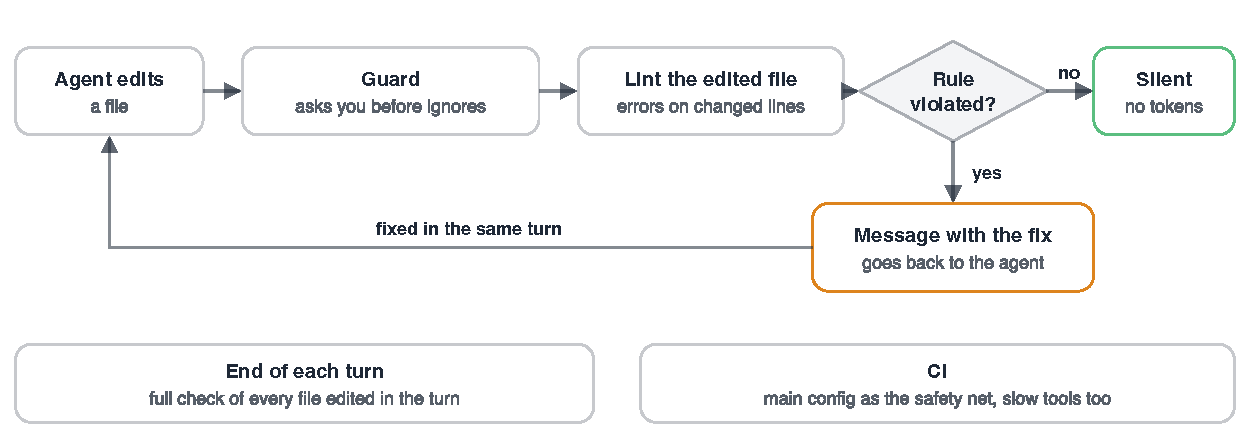
\includegraphics[width=\linewidth]{generated/fig2-loop.pdf}
\caption{The in-session feedback loop of the \arm{rules} arm. After each edit, a guard and the linter run on the edited file. A clean result costs no tokens. A violation returns a message with the fix, and the agent usually fixes it in the same turn. A full check runs at the end of each turn.}
\label{fig:loop}
\end{figure}


We separate two kinds of rules.
A \emph{mechanical} rule changes one expression, for example \texttt{status.HTTP\_404\_NOT\_FOUND} instead of \texttt{status\_code=404}.
A \emph{design-shaping} rule changes where code goes, for example a success notification in the mutation hook instead of in the component.
A mechanical rule is cheap to fix late.
A design-shaping rule is not: a late fix means that the agent must move code that it already wrote.
The pointer exists for this second kind, because it tells the agent the right shape before it writes.
Figure~\ref{fig:example} shows one rule in its three forms.

\begin{figure}[!htb]
\small
\textbf{Prose} (one bullet in the middle of a list in \file{docs/backend.md}):
\begin{quote}\ttfamily\footnotesize
- Time: inject `java.time.Clock` and call `Instant.now(clock)`\\
\hspace*{1em}(or the matching `now(clock)`); never call `now()` without a clock.
\end{quote}
\textbf{Lint rule} (ast-grep; the message goes to the agent):
\begin{quote}\ttfamily\footnotesize
id: use-clock-injection\\
language: Java\\
severity: error\\
message: \$T.now() without a Clock. Inject java.time.Clock and call \$T.now(clock).\\
rule: \{ pattern: \$T.now() \}\\
constraints: \{ T: \{ regex: (Instant|LocalDate|...)\$ \} \}
\end{quote}
\textbf{Pointer} (one line in \file{src/main/java/CLAUDE.md}):
\begin{quote}\ttfamily\footnotesize
- Time: inject `java.time.Clock` and call `now(clock)`; never `now()` without\\
\hspace*{1em}a clock (enforced by use-clock-injection).
\end{quote}
\textbf{Task prompt} (the same in every arm; it does not name the rule):
\begin{quote}\ttfamily\footnotesize
Add an admin-only REST endpoint GET /api/admin/users/recently-created that\\
returns the logins of users created in the last 7 days. Put the query in the\\
user repository and the logic in the user service. Do not run the build.
\end{quote}
\caption{One design-shaping rule of the jhipster study in its three forms, and one task prompt. The regular expression is shortened.}
\label{fig:example}
\end{figure}

The \arm{rules} arm is the setup that the open-source tool codemyrules installs.
The author of this paper also wrote codemyrules (see the conflict-of-interest statement).

\section{Method}
\label{sec:method}

\subsection{Harness}

agent-rules-bench has four steps (Figure~\ref{fig:bench}).
\textbf{prepare} clones the repository once per arm at the pinned commit, runs the setup script of the arm, and tags the result.
\textbf{run} resets the copy before every session and starts one headless agent session.
For Claude Code this is \texttt{claude -p} with project settings only, so the personal hooks and plugins of the experimenter have no effect.
The study sets the model, the allowed tools and a turn cap (30 in most studies, 60 on Formbricks).
After each session the harness runs the checkers of the study on the lines that the agent added.
The checkers are the same for every arm and live outside the copies, so no arm is measured with its own rules.
If a run violated a rule, one more session gives the agent precise review feedback, with the same text in every arm.
\textbf{verify} applies the final diff of each run to a clean checkout of the pinned commit, without the setup of any arm, and runs the build and the tests of the project.
\textbf{summarize}, \textbf{compare} and \textbf{pool} produce the statistics.
The harness needs only Node.js and git, and its own test suite runs against a fake agent.

\begin{figure}[!htb]
\centering
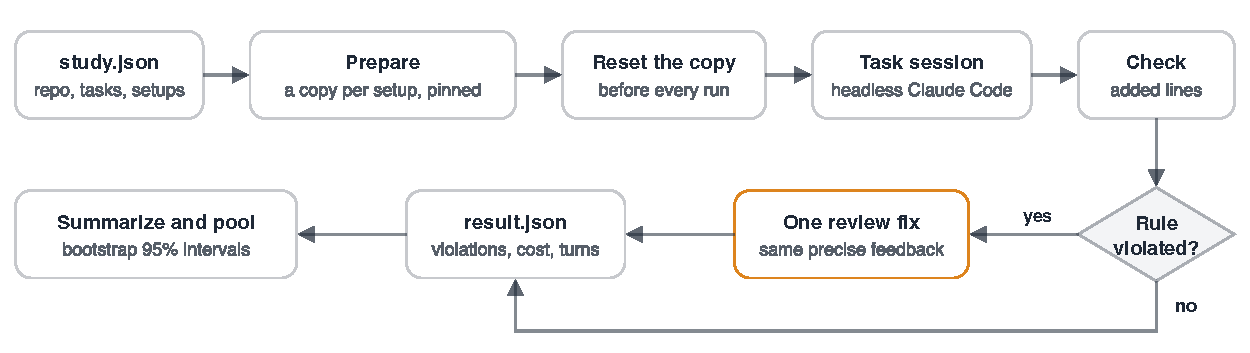
\includegraphics[width=\linewidth]{generated/fig3-bench.pdf}
\caption{One run in agent-rules-bench. Every session starts from a fresh copy of its arm. A run that violated a rule gets one review-fix session.}
\label{fig:bench}
\end{figure}

\subsection{Projects, rules and tasks}

Table~\ref{tab:projects} lists the four public projects.
In each project the existing code already violates the rules: jhipster calls \texttt{Instant.now()} 7 times, the FastAPI routes call the database session 32 times, and all 7 bulletproof-react feature components with a mutation call the notification hook themselves.
An agent that copies nearby code therefore violates the rule.
We chose this design on purpose, because it makes a missed rule visible.
It also means that our violation rates are an upper bound for everyday work (Section~\ref{sec:threats}).

\begin{table}[!htb]
\centering
\small
\caption{Projects and rules. D = design-shaping, M = mechanical.}
\label{tab:projects}
\begin{tabularx}{\linewidth}{@{}lLL@{}}
\toprule
Project (language, checker) & Rules & Tasks \\
\midrule
jhipster-sample-app (Java, ast-grep) & D: inject a \texttt{Clock}, no \texttt{Instant.now()}. M: authorities from constants, no \texttt{"ROLE\_ADMIN"}. & Admin-only endpoints over the last 7 and 30 days. \\
full-stack-fastapi-template (Python, ast-grep) & D: database access only in \file{crud.py}. M: status-code constants, no integer literals. & Per-user item statistics; clear an item's description with owner checks. \\
bulletproof-react (TypeScript, ESLint) & D: success notifications in the mutation hook. M: query keys from query options. Plans 4--6: 40 conventions. & Edit a comment; change a user's role; rename a team; create teams; four tasks outside all conventions. Plan~6: pin discussions; comment counts; change password; filter and export users. \\
Formbricks (TypeScript, ESLint) & Plan~6: 4 conventions in the maintainers' words; D: no new server actions. M: \texttt{Readonly<>} props; shared date formatting; strings only in \texttt{en-US.json}. & API keys, webhooks, profile and tags: two features each. \\
\bottomrule
\end{tabularx}
\end{table}


Plans 4 and 5 use a list of 40 conventions for bulletproof-react.
The conventions cover architecture, the API layer, authorization, UI, routing, TypeScript, files and the mock API.
Each convention has one prose line, and the same line is its lint message and the text of its review fix.
Prose and lint rule therefore state each convention in the same words.

Plan~6 adds Formbricks, an open-source survey platform, at a pinned commit.
Its conventions are not ours: we took them word for word from the maintainers' \file{AGENTS.md} and \file{CODING\_STANDARDS.md}, and we used only the four that its own ESLint configuration does not enforce.
The existing code violates three of them: it has 57 files with server actions, and 383 components without \texttt{Readonly<>} props.
Claude Code loads \file{AGENTS.md} in every session, but it loads \file{CODING\_STANDARDS.md} only if the agent opens it.
So in the prose arm of Formbricks, two conventions (F1, F4) are always loaded and two (F2, F3) are in a document that the agent may not open.
We kept the files as the maintainers wrote them.

\subsection{Measures}

A \emph{violation} is a checker finding on an added line in production code, after the task session and before any review fix.
A run is \emph{violating} if it has at least one violation.
\emph{Cost} is the total cost per run that Claude Code reports: the task session plus the review fix, if there was one.
Cost combines tokens, turns, cache use and rework in one number.
We also record turns, tokens, wall time, loop catches, the violations left at the end and the verify result.

\subsection{Models and agents}

The Claude Code runs of the exploratory studies and of Plans 1 to 5 use \texttt{claude-sonnet-5-5} and \texttt{claude-haiku-5-5}.
We read the model identifiers from the session output.
These runs took place between 1 and 5 November 2026, and the \NClaudeRuns{} runs cost \TotalCost{} in total.

Plan~6 uses the same two models as its primary models (Claude Code 2.1.325) and ran between 15 and 17 November 2026.
As a second model family it uses \texttt{qwen3.6:35b-a3b-coding} in the Codex CLI 0.166.0 with the same feedback loop.
A deviation added exploratory runs with the two newest Claude models, \texttt{claude-opus-5-5} and \texttt{claude-fable-5-2}, with 1 or 2 repeats per cell.
Each Plan~6 run records the agent version, the model identifiers and the commit of the harness.
The Claude Code runs of Plan~6 cost \PSixCost{} in total.

One exploratory study also repeats a comparison with a local model, \texttt{qwen3.6:35b-a3b} (Q4\_K\_M quantization), in two other agents, pi and the Codex CLI, with the same feedback loop.
These runs have a turn cap of 60, because the local model needs more turns than the Claude models.
A local model reports no cost, so for these runs we report violations and turns only.

\subsection{Use of AI tools in this work}

AI coding agents are the subject of this study, and this section describes how they were run.
Apart from that, the author used Claude (Anthropic) in Claude Code to write and test the code of the harness and the analysis scripts, to operate the runs, and to draft and edit the text of this paper.
The hand labels of the measurement checks are the author's own judgments: the labelling page showed each finding or diff with the convention text and the arm hidden, and recorded only the author's answer.
The author reviewed all code, analyses and text, and is responsible for the content.

\subsection{Exploratory and pre-registered studies}

The work has two phases, and we keep them apart in all results.

In the first phase we ran four \emph{exploratory} studies.
They had no fixed analysis plan, because their purpose was to form ideas.
While we ran them, we also completed the harness: the arms, the checkers, the review fix and the measures took their final form in this phase.
These studies gave us the questions that the second phase tests, for example what the loop and the pointer each contribute, and what a large always-loaded file costs.
We report their results as exploratory, and we draw no confirmatory conclusion from them.

In the second phase we tested these ideas.
We wrote six analysis plans, Plans~1 to~6, one for each new study.
We committed each plan to the public repository before the first run of its study \citep{nosek2018prereg,ernst2023registered}.
The commit history therefore shows that each plan is older than its data.
This is what we mean by \emph{pre-registered}: we fixed the arms, outcomes, hypotheses and statistical tests of a study before we saw any of its results.
Each plan also lists every later deviation with its date.
Only the hypotheses of these plans are confirmatory (Tables~\ref{tab:hyp} and~\ref{tab:plan6}).

Plan~6 is stricter than Plans 1 to 5 in four ways.
We registered it on OSF before its first run (\url{https://osf.io/9hdjs}), and it lists five deviations, each with its date, its reason and what we knew when we made it.
Its sample size comes from a power analysis: 128 runs per arm give 80\% power for 8\% against 1\% violating runs (one-sided exact test, $\alpha=0.05$).
A seed interleaves the arms in time, so that no arm runs as one block with a warm prompt cache.
Install, build and verify run in a container without credentials.

\subsection{Statistics}

For violations we use the exact conditional Cochran--Mantel--Haenszel test \citep{mantel1959}, one-sided and stratified by study and model.
With one stratum it is Fisher's exact test.
For cost we use the geometric mean of the per-stratum ratios of mean cost, with a 95\% stratified bootstrap interval (10{,}000 resamples, fixed seed) \citep{efron1993bootstrap} and a one-sided bootstrap $p$.
Within one plan we correct the hypotheses with Holm's method \citep{holm1979} at a family-wise $\alpha=0.05$.
For the cost hypothesis of Plan~6 (H13) we test equivalence with two one-sided tests \citep{schuirmann1987tost,lakens2017equivalence}: it holds if the 90\% stratified bootstrap interval of the cost ratio lies inside 0.90 to 1.10.
Plan~1 is the exception: it tests its two hypotheses separately, as the plan states.
Verify pass rates have exact Clopper--Pearson intervals \citep{clopper1934}.
A script generates every table and every number in this paper from the published results.

\section{Results}
\label{sec:results}

\subsection{Exploratory studies}

Table~\ref{tab:pooled} pools the four exploratory studies, and Appendix~\ref{app:per} lists each comparison.

\begin{table}[!htb]
\centering
\footnotesize
\setlength{\tabcolsep}{3pt}
\caption{Exploratory studies: \arm{rules} against prose. Cost change is rules/prose with a 95\% bootstrap interval; violating = runs with a violation after the task. One FastAPI comparison is excluded, because those Sonnet runs skipped the linked documents and wrote no tests, so they did less work. With it, always-loaded prose vs.\ rules is +10\% ($-$1\% to +22\%) for all models. Violations in jhipster-buried include new test files, which its documents did not cover; in production code only, its prose arms violated the rule in 0/8 (Sonnet) and 3/8 (Haiku) runs, so prose the agent can miss was violated in 11/56 runs.}
\label{tab:pooled}
\begin{tabular}{@{}llcccrr@{}}
\toprule
Rule location & Model & Cells & Prose violating & Rules violating & Cost & 95\% CI \\
\midrule
\rows{generated/pooled.tex}
\bottomrule
\end{tabular}
\end{table}


\paragraph{Prose that the agent can miss.}
When the rule was in linked or buried prose, the agent violated it in \PoolMissProse{} runs.
When the same rule was a lint rule, the agent violated it in none.
The cost change was \PoolMissCost{} (\PoolMissCI), because no run with lint rules needed a review fix.
Haiku missed buried prose more often (13 of 24 runs) than Sonnet (4 of 32).
Almost every violation was of a design-shaping rule, and the agent had copied the violating pattern from nearby code.

\paragraph{Prose that the agent reads.}
When the rule was in a short always-loaded \file{CLAUDE.md}, the agent followed it in all runs, as it did with the lint rule, and at equal cost.
A short document behind one clear link was also followed in every run (jhipster, 8 of 8).
Prose therefore fails when it is buried among other text, not because it is prose.

\paragraph{A side effect of always-loaded rules.}
With the rules in \file{CLAUDE.md}, Sonnet on FastAPI stopped opening the linked documents.
It then wrote no tests in any run, so it missed the testing convention that only those documents state.
Always-loaded text can change what else the agent reads.

\subsection{Pre-registered studies}

The five pre-registered studies test the ideas that the exploratory studies gave us.
Table~\ref{tab:hyp} gives every pre-registered hypothesis with its result.
Of the nine hypotheses of Plans 1 to 5 that we could test, three are supported.
H3 has no test by design, and H4 could not be tested.

\begin{table}[!htb]
\centering
\footnotesize
\setlength{\tabcolsep}{4pt}
\caption{Pre-registered hypotheses. Violations: violating runs in the first arm vs.\ the second. Cost: change with 95\% stratified bootstrap interval. $p$: exact one-sided CMH (violations) or one-sided bootstrap (cost). Verdicts apply Holm's correction within each plan. H3 is descriptive: it gives the runs whose production code passes the original test suite.}
\label{tab:hyp}
\begin{tabularx}{\linewidth}{@{}lcLLlll@{}}
\toprule
& Plan & Claim & Comparison & Result & $p$ & Supported \\
\midrule
\rows{generated/hypotheses.tex}
\bottomrule
\end{tabularx}
\end{table}

We report the other six in full, because a null result here is also information for practice.

\paragraph{What the loop and the pointer do (Plan 1, 144 runs).}
Three arms differ in one part each: the full setup, the setup without the loop (\arm{pointer\_only}), and the setup without the pointer (\arm{rule\_only}).
Without the loop, \HOneBreaks{} runs violated a rule, against \HOneBreaksAgainst{} with it (H1 supported).
All 8 violations were of the mechanical status-code rule on FastAPI.
This rule had no pointer line, so no text stated it at all.
The three design-shaping rules, each with its pointer line, were violated in 0 of 48 runs without the loop.
The measured value of the loop is therefore that it enforces rules that no prose states.

Without the pointer, the loop caught the design-shaping rule \HTwoCatchNoPointer{} times, against \HOneCatchFull{} times with it, and the cost change was \HTwoCost{} (\HTwoCI; H2 supported).
With the pointer, the agent writes the right shape first.
With the loop alone, the agent reaches the same result through rework.

H3 states that functional correctness does not differ between the three arms, and the plan gives it no test.
The production code passed the original test suite in \HThreeNoLoop{} runs without the loop (exact 95\% interval \HThreeNoLoopCI), in \HThreeNoPointer{} runs without the pointer (\HThreeNoPointerCI) and in \HThreeFull{} runs with the full setup (\HThreeFullCI).

\paragraph{Missed rules over a sequence of sessions (Plan 2).}
This plan ran three tasks in a row on the same copy, to test whether a missed rule compounds.
The usage limit of the account stopped \the\numexpr\SeqPlanned-\SeqOk\relax{} of its \SeqPlanned{} sessions, including all Haiku chains.
The complete Sonnet sessions show no violation in either arm (\HFourBreaks{} vs.\ \HFourBreaksAgainst{} in T2 and T3).
These data cannot test the hypothesis, and we report H4 as not tested.
Plan~2 also named a small descriptive study with a stronger model (Claude Opus, 16 runs, no hypothesis).
We dropped it before any of its runs, because it asks how strong a model must be to follow buried prose, which is a different question.
Plan~3 took its place, and the plan records this change with its date.

\paragraph{A large always-loaded file (Plan 3, 64 runs).}
Teams often put all their documents into the always-loaded file.
We put the project's own \file{AGENTS.md} and its nine guides into \file{CLAUDE.md}, which gives 15.7k tokens in every session, with the two rules in the same positions as in \arm{prose\_buried}.
Against lint rules with short documents, the cost change was \HSixCost{} (\HSixCI, $p=\HSixCostP$; H6 supported).
The large file had \HFiveBreaks{} violating runs against \HFiveBreaksAgainst{} (all Haiku, $p=\HFiveBreaksP$; H5 not supported at 16 runs per arm).
The same rule sentence was followed in a short \file{CLAUDE.md} in all 16 runs.

\paragraph{Forty conventions (Plan 4, 96 runs).}
We stated 40 conventions as 40 prose lines in a short always-loaded file (757 words, 1.9k tokens), and compared them with 40 lint rules and 8 pointers.
The result was even: \HSevenBreaks{} vs.\ \HSevenBreaksAgainst{} violating runs ($p=\HSevenBreaksP$) and a cost change of \HEightCost{} (\HEightCI).
Neither hypothesis is supported.

Stating the conventions mattered in either form.
Without them, every run violated at least one convention, and the review fix gave a cost change of \NoneVsProseCost{} (\NoneVsProseCI).
Only 4 of the 40 conventions were ever violated.
The agent followed the other 36 because the code around it already followed them.
In the \arm{rules} arm, the agent wrote a violation in 13 of 32 runs; each time the loop caught it and the agent fixed it in the same session.

\paragraph{Conventions among business context (Plan 5, 288 runs).}
A real \file{CLAUDE.md} also holds product context.
Every arm got 1,328 words of business context, and the prose arm added the 40 lines.
On the feature tasks, prose was violated in \HNineBreaks{} runs and lint rules in \HNineBreaksAgainst{} ($p=\HNineBreaksP$), with a cost change of \HTenCost{} (\HTenCI).
On four tasks outside the scope of every convention, the 1.9k tokens of prose gave a cost change of \HElevenCost{} (\HElevenCI).
H9 to H11 are not supported.
With a warm prompt cache, the measured extra cost of the prose was about 4\% of a short Sonnet session.
This is close to the price that the token counts predict, and it is too small to detect with 64 runs per arm.

\subsection{Conventions on two projects (Plan 6)}
\label{sec:plan6}

Plans 4 and 5 each came out even, but pooled after the fact they gave 7 violating runs with prose against none with lint rules.
Plan~6 tests this as a confirmatory hypothesis, on two projects, with a second model family.
In bulletproof-react the 40 conventions are in a short always-loaded \file{CLAUDE.md}, as in Plan~4, with four new tasks.
In Formbricks the four conventions are in the maintainers' own files (Section~\ref{sec:method}).
In the \arm{rules} arm the convention lines are removed from these files, and each convention is a lint rule with the feedback loop.
Table~\ref{tab:plan6} gives every stratum.

\begin{table}[!htb]
\centering
\small
\caption{Plan~6: violating runs per stratum, with a one-sided Fisher test, and the change in mean total cost (rules/prose). Upper part: primary models (H12, H13). Lower part: the local model in Codex (H14, secondary; no cost).}
\label{tab:plan6}
\begin{tabular}{@{}llccrr@{}}
\toprule
Project & Model & Prose violating & Rules violating & $p$ & Cost \\
\midrule
\rows{generated/plan6.tex}
\bottomrule
\end{tabular}
\end{table}

\paragraph{Violations (H12, not supported).}
Over both projects and both Claude models, prose was violated in \HTwelveProse{} runs and lint rules in \HTwelveRules.
The exact stratified test gives $p=\HTwelveP$, and $p=\HTwelveHolm$ after Holm's correction with H13, so H12 is not supported.
The pooled result hides a split by project.
On Formbricks, prose was violated in \PSixFBProse{} runs and lint rules in \PSixFBRules{} ($p$~\PSixFBP, not corrected).
On bulletproof-react the two arms were even, \PSixBPProse{} against \PSixBPRules.

\paragraph{Formbricks: prose that is not loaded.}
Table~\ref{tab:formbricks} splits Formbricks by convention.
Most violations of prose were of F2 and F3, the two conventions in \file{CODING\_STANDARDS.md}, which Claude Code does not load by itself.
With lint rules, these two were violated in no run.
F1, the design-shaping rule against new server actions, is in the always-loaded \file{AGENTS.md}; the Claude models rarely violated it in either arm.
F4 was violated in no run.
This is the pattern of the exploratory studies: lint rules help where the agent does not read the prose.

We also checked in the session logs whether each prose run opened \file{CODING\_STANDARDS.md} (exploratory).
The Claude models opened it in \PSixOpened{} runs.
F2 or F3 was violated in \PSixOpenedViol{} of the runs that opened it and in \PSixNotOpenedViol{} of the runs that did not.
Opening the document therefore helped little.
The logs do not show whether the agent read the part of the document that states the convention.

\begin{table}[!htb]
\centering
\small
\caption{Plan~6, Formbricks: runs with a violation of each convention, by where the prose arm states it (loaded: \file{AGENTS.md}, which \file{CLAUDE.md} imports; not loaded: \file{CODING\_STANDARDS.md}). Claude: Sonnet 5.5 and Haiku 5.5 together.}
\label{tab:formbricks}
\setlength{\tabcolsep}{4pt}
\begin{tabular}{@{}lllcccc@{}}
\toprule
& & Prose & \multicolumn{2}{c}{Claude} & \multicolumn{2}{c}{Qwen3.6} \\
& Convention & location & prose & rules & prose & rules \\
\midrule
\rows{generated/plan6-formbricks.tex}
\bottomrule
\end{tabular}
\end{table}

\paragraph{bulletproof-react: one convention, one task.}
All violating runs of bulletproof-react broke one convention, ``role checks go through the authorization helpers'' (\PSixBPRoleRuns{} violating runs), and all of them in task T4 (\PSixBPRoleTFour), which asks for a filter of the users list by role.
The code that the task asks for compares a user's role with the selected role.
The checker cannot tell a filter from an access check, and the existing code does not show which form the convention expects.
In the \arm{rules} arm the loop reported a finding in \PSixBPCatchRuns{} runs.
In \PSixBPIgnoredRuns{} runs the agent kept the flagged code after the loop had reported it, which the message of the loop allows when the agent thinks the code is legitimate.
So on bulletproof-react the agent saw the convention in both arms: as always-loaded prose, or as a message of the loop.
In both arms it often judged the filter as allowed, and the arms came out even.

\paragraph{Cost (H13, not supported).}
Lint rules changed the cost by \HThirteenCost{} against prose (90\% interval \HThirteenCI).
The interval is not inside the margin of $\pm$10\%, so equivalence is not shown ($p=\HThirteenP$).
Without the review fix the change was \HThirteenTaskCost{} (\HThirteenTaskCI).
The strata point in different directions, from $-$16\% to +29\% (Table~\ref{tab:plan6}).
On bulletproof-react with Sonnet, the \arm{rules} arm cost more, and its runs took more turns.

\paragraph{A second model family (H14).}
With the local model in Codex, lint rules reduced the violating runs from \HFourteenProse{} to \HFourteenRules{} ($p$~\HFourteenP).
The model violated prose on both projects, also the always-loaded prose of bulletproof-react.
On Formbricks, its remaining violations with lint rules were all of F1 (Table~\ref{tab:formbricks}): the loop reported the new server action, and the model kept it.
A design-shaping rule asks the agent to move code it already wrote, and this model did not do that.

\paragraph{Functional correctness (H15).}
Table~\ref{tab:plan6verify} gives the verify pass rates.
The arms did not differ.
Two project tests fail for any correct solution of their task: in bulletproof-react T2 a test finds table rows by their full text, and in Formbricks T1 a test expects the exact database query.
We wrote a minimal correct solution for every task by hand, ran it through verify, and left out the project test files that it fails (deviation D5).
With that, the pass rates rise, and the arms still do not differ.

\begin{table}[!htb]
\centering
\small
\caption{Plan~6: runs whose final diff passes the type check and the project's tests on the unchanged commit (primary models). D5: without the test files that a hand-written correct solution also fails.}
\label{tab:plan6verify}
\begin{tabular}{@{}lcccc@{}}
\toprule
& \multicolumn{2}{c}{As registered} & \multicolumn{2}{c}{D5} \\
Project & Prose & Rules & Prose & Rules \\
\midrule
\rows{generated/plan6-verify.tex}
\bottomrule
\end{tabular}
\end{table}

\paragraph{The newest models (exploratory).}
Table~\ref{tab:latest} gives the runs with Claude Opus 5.5 and Fable 5.2 (deviation D1).
They violated few conventions in either arm, and none on Formbricks.
On bulletproof-react, Fable 5.2 needed about twice as many turns with lint rules, because it read more files and reacted to the messages of the loop.
With 1 or 2 repeats per cell these runs support no test.

\begin{table}[!htb]
\centering
\footnotesize
\setlength{\tabcolsep}{4pt}
\caption{Plan~6, exploratory: the newest Claude models (descriptive only).}
\label{tab:latest}
\begin{tabular}{@{}llcccc@{}}
\toprule
& & \multicolumn{2}{c}{Violating} & \multicolumn{2}{c}{Mean turns} \\
Project & Model & Prose & Rules & Prose & Rules \\
\midrule
\rows{generated/plan6-latest.tex}
\bottomrule
\end{tabular}
\end{table}

\paragraph{Measurement checks.}
The author labelled by hand, with the arm hidden, a random sample of 40 diffs per project for every convention in scope of the changed files, and every finding that the loop reported.
On Formbricks the checkers agreed with the labels: precision \PSixFBPrecision{} and recall \PSixFBRecall{} over \PSixFBCells{} labelled cells.
On bulletproof-react they agreed less: precision \PSixBPPrecision{} (\PSixBPPrecisionCI) and recall \PSixBPRecall{} (\PSixBPRecallCI) over \PSixBPCells{} cells.
All \PSixBPFpRole{} findings that the labels did not confirm were role checks on code that offers an ``all roles'' choice in a filter.
Of the cells that only the labels marked, \PSixBPFnNoAny{} were \texttt{any} types in the mock API handlers, a folder outside the scope of the lint rule, \PSixBPFnZod{} were input types written by hand instead of derived from the schema, and \PSixBPFnOther{} were other conventions.
These misses affect both arms alike, because one checker measures both.
Of the findings that the loop reported in the \arm{rules} arm, \PSixLoopFalse{} were labelled false (\PSixLoopFalseCI), and of the findings after the task in both arms, \PSixAfterFalse{} (\PSixAfterFalseCI).
Without these false findings H12 does not change (deviation D2).
The lint rules took \PSixBPLOC{} lines of rule code and \PSixBPCases{} test cases for the \PSixBPConventions{} conventions of bulletproof-react, and \PSixFBLOC{} lines and \PSixFBCases{} test cases for the \PSixFBConventions{} of Formbricks.

\subsection{Descriptive and post hoc comparisons}

Table~\ref{tab:desc} lists the comparisons that the plans name as descriptive.
Two of them matter for the discussion.

\begin{table}[!htb]
\centering
\footnotesize
\setlength{\tabcolsep}{3pt}
\caption{Comparisons the plans list as descriptive, without hypothesis tests, and one pooling chosen after the results.}
\label{tab:desc}
\begin{tabularx}{\linewidth}{@{}Lllll@{}}
\toprule
Comparison & Arms & Violating & $p$ & Cost [95\% CI] \\
\midrule
\rows{generated/descriptive.tex}
\bottomrule
\end{tabularx}
\end{table}


First, the same rule sentence was followed in the short file and violated in the large file (3 of 16 runs, all Haiku).
This points to dilution, but the difference is not significant.

Second, Plans 4 and 5 together give \PoolFourFiveBreaks{} violating runs with prose against none with lint rules ($p=\PoolFourFiveP$), at equal cost.
We chose this pooling after we saw both results.
It is therefore a reason to run a confirmatory study, and it does not replace one.
Plan~6 is that study, and it did not confirm the pooled result (Section~\ref{sec:plan6}).

\subsection{Functional correctness}

A rule setup must not make the code worse.
\textbf{verify} built and tested the final diff of each run on the plain upstream commit.
In the exploratory studies and Plans 1 to 5, the production code passed the original test suite of the project in \NVerifyOk{} of \NClaudeRuns{} runs, and the arms did not differ (Plan~6: Table~\ref{tab:plan6verify}).
The \NVerifyFail{} failures are type errors and compile errors that are unrelated to the rules; \NVerifyHaikuFail{} of them come from Haiku.

\subsection{Other agents and a local model}

Table~\ref{tab:local} shows \NLocalRuns{} exploratory runs with a local model in pi and Codex (Plan~6 repeats this in Codex as a registered secondary hypothesis, Section~\ref{sec:plan6}).
These agents load only the root \file{AGENTS.md} by themselves and never load a folder-level pointer.
In these runs, \arm{prose\_buried} therefore means documents that the agent must find without help.

\begin{table}[!htb]
\centering
\small
\caption{Exploratory: a local model (qwen3.6, 35B, quantized) in pi and Codex on bulletproof-react, 8 runs per cell. $p$: one-sided Fisher against \arm{rules}.}
\label{tab:local}
\begin{tabular}{@{}llcrr@{}}
\toprule
Agent & Arm & Violating & $p$ & Mean turns \\
\midrule
\rows{generated/local.tex}
\bottomrule
\end{tabular}
\end{table}


With prose in documents, every run violated the design-shaping rule in both agents.
With lint rules and the loop, pi had no violating run and Codex had one.
The same rule text in the always-loaded \file{AGENTS.md} did not help in pi (8 of 8 runs violating) and helped partly in Codex (3 of 8).
In pi, the \arm{rules} arm needed about half the turns of the prose arms.
These runs show that the feedback loop carries over to other agents.
They say little about local models in general.
H14 in Plan~6 confirms the direction on two projects.

\subsection{Rules that the tool builds}

In the main studies we wrote the lint rules by hand.
As a check of the tool, we also ran the rules that codemyrules built by itself from the \arm{prose\_buried} state of three studies.
These generated rules had \GenBreaks{} violating runs in production code.
Against the hand-written rules, the cost change was \GenCost{} (\GenCI).
Part of this difference comes from less work, because these runs wrote tests less often.
This check is not part of the main question.

\section{Discussion}
\label{sec:discussion}

\paragraph{Where prose fails.}
Prose that the agent reads works.
A short always-loaded file and a short document behind one clear link were followed as well as lint rules.
This agrees with \citet{gloaguen2026agentsmd}, who report that agents follow the instructions in context files well.
Prose fails when the agent does not read it: a bullet in the middle of long linked documents, or a document that the agent never opens.
The failures are not random.
In the exploratory studies they are design-shaping rules for which the existing code shows the wrong pattern, and the weaker model copies that pattern more often.
Plan~6 shows the same split with conventions that a project's maintainers wrote.
On Formbricks, two conventions sit in a document that Claude Code does not load, and lint rules removed almost all violations of them.
On bulletproof-react, all 40 conventions are in a short always-loaded file, and lint rules gained nothing.
The registered test pools the two projects, and it is not significant after correction.
We read this as one result, not two: the gain of a lint rule depends on whether the agent reads the prose, and the pooled test averages a project where it does not with one where it does.

\paragraph{What the lint rule adds.}
A lint rule does not depend on the attention of the agent.
Of the \NLoopRuns{} Claude Code runs with the feedback loop in the exploratory studies and Plans 1 to 5, \NLoopBroken{} ended the task with a violation in production code.
This is cheap when the agent already follows the rule, because a passing check sends nothing to the model.

\paragraph{What the lint rule does not add.}
The loop reports; it does not force.
Plan~6 shows two cases where the agent saw the message and kept the code.
On bulletproof-react, the task asked for a role filter, the checker flagged it as an access check, and the agent kept it in \PSixBPIgnoredRuns{} runs.
The hand labels did not settle whether this code violates the convention.
On Formbricks, the local model kept new server actions after the loop had reported them.
A lint rule therefore does not help when the agent disagrees with it, or when following it means moving code that the agent has already written.
In the first case the rule or its message must be more precise.
In the second case the pointer did not prevent it: F1 had a pointer line in \file{AGENTS.md}, and the local model still wrote the server action first.
Writing the lint rules also has a cost: \PSixBPLOC{} lines and \PSixBPCases{} test cases for 40 conventions, against 40 lines of prose.
The ablation shows how the two parts share the work.
The loop enforces rules that nobody wrote down.
The pointer prevents the rework that a late catch of a design-shaping rule causes.

\paragraph{What always-loaded prose costs.}
The token price of a short always-loaded file is small: about \$0.006 per 1k tokens per Sonnet session at median turns, and less with a warm cache.
We could not separate 1.9k tokens of prose from noise.
The cost becomes measurable when the file grows: at 15.7k tokens the cost change was \HSixCost{}.
The risk of a missed rule may also grow: the same rule was followed in the short file and violated in 3 of 16 runs with the large one.
This difference is not significant, and \citet{mcmillan2026adherence} finds no effect of file size on adherence, so we do not claim it.

\paragraph{A guideline.}
From these results we suggest four practices:
\begin{enumerate}
\item Put a rule that a linter can check, and that the agent may not read, into a lint rule, and run it in an in-session feedback loop, not only in CI.
A rule in a document that the agent does not load is the first candidate.
\item For a design-shaping rule, add a one-line pointer near the code where the rule applies.
\item Keep the always-loaded file short, and link each longer document with one clear sentence.
\item Do not expect the agent to follow a rule in the middle of long documents, above all when the existing code violates it.
\item Write the message of a lint rule so that the agent cannot read a legitimate exception into it, and check the rule on the tasks it will see: a rule that flags code the task asks for is ignored, and costs turns.
\end{enumerate}

\section{Threats to Validity}
\label{sec:threats}

\paragraph{Adversarial tasks.}
We designed the tasks so that an agent that copies nearby code violates a rule.
Our violation rates are therefore an upper bound.
We did not measure how often natural tasks touch the scope of a rule.
Tasks mined from merged pull requests would answer this question.

\paragraph{Few projects and rules.}
We used four projects, and Plans 2 to 5 used only one of them.
Plan~6 used two, and they gave opposite results.
They differ in more than one way: where the prose is (loaded or not), the number of conventions (40 against 4), who wrote the conventions, and how well the checkers measure them.
With two projects we cannot tell which difference matters; the per-convention split of Formbricks points to the first.
The author wrote the 40 conventions of bulletproof-react and its business context from the documents and the code of the project.
Only a few of the 40 conventions were ever at risk in the tasks, and in Plan~6 one convention in one task explains every violation.

\paragraph{Sample size.}
Most cells of Plans 1 to 5 have 8 runs, and the cost varies widely between runs of the same arm.
Several null results (H5, H7, H9) can only exclude large differences.
Plan~6 has 128 runs per arm and a power analysis, but its expected effect assumed that violations spread over many conventions.
They are not evidence of equal compliance.

\paragraph{Measurement.}
The checkers define what a violation is, so their blind spots are ours.
In jhipster-buried the checkers also covered test files, which the documents did not.
The exploratory pool counts those violations (17/56 runs, 11/56 in production code only), and all later studies count production code only.
For the exploratory studies and Plans 1 to 5 we did not measure the false-positive rate of the lint rules.
In Plan~6 we labelled every loop finding and a blind sample of diffs.
One author did all labels with the arm hidden, and there was no second rater.
The checkers of bulletproof-react had a low recall in the sample (\PSixBPRecall), mostly because of a scope that leaves out the mock API; this lowers the violation counts of both arms alike.
The diff labels and the finding labels disagree on the role-filter pattern: the diff labels judge \PSixBPFpRole{} of these findings as no violation, while the finding labels mark only \PSixAfterFalse{} findings as false.
The review fix is idealised: one precise prompt, no human time and no CI round trip.
Real review costs more, which would favour arms with fewer violations.

\paragraph{Cost and reach of lint rules.}
We measured the size of the lint rules of Plan~6 (lines and test cases), but not the time to write and maintain them, which is higher than the time to write one sentence.
Not every rule can become a lint rule: a rule about intent, or about a design choice across many files, may have no pattern that a linter can check.
Our results apply to rules that a linter can check.

\paragraph{Models and agents.}
We used four Claude models in Claude Code and one local model in two other agents, in the versions that were current in November 2026.
For the studies before Plan~6 we did not record the exact tool versions at run time, and sessions of one arm ran back to back and shared the prompt cache.
Plan~6 records the versions and interleaves the arms.
Updates of a model or an agent can change the results.
Repeated runs of the same prompt give different code \citep{ouyang2025nondeterminism}, which is why every cell of our studies has several repeats.
The Claude models are closed, so we cannot rule out that their training data contains the public projects that we used \citep{sallou2024threats}; we follow the published guidelines for empirical studies with language models where they apply \citep{baltes2025guidelines}.

\paragraph{Incomplete plan.}
Plan~2 stopped at the usage limit of the account, and we report it as not tested.

\paragraph{Conflict of interest.}
The author wrote codemyrules, which installs the \arm{rules} arm.
To limit this bias, we committed the plans before the runs and registered Plan~6 on OSF, we used the same checkers for all arms, we publish every run, and we report the null results of the pre-registered studies in full.

\section{Conclusion}

We compared the places where a coding rule for AI coding agents can live.
Prose works when the agent reads it.
A lint rule with an in-session feedback loop works whether or not the agent reads anything, and it costs nothing while the code is correct.
Lint rules show their clearest gains against prose that the agent can miss, against large always-loaded files, and with a weaker model.
Against short always-loaded prose, the two come out even in our pre-registered tests.
Our largest registered study did not confirm a general advantage of lint rules: they helped on the project whose prose the agent did not load, and not on the project whose prose it always loaded.
A lint rule reports, and the agent can still keep code that it thinks is right.
The harness and all \NTotalRuns{} runs are public, so others can test other projects, rules and agents.

\backmatter

\section*{Statements and Declarations}

% The declarations of the EMSE version, used in main-emse.tex and in title-page-emse.tex.
\begin{itemize}
\item \textbf{Funding:} This work had no external funding.
\item \textbf{Competing interests:} The author is the developer of codemyrules (\url{https://github.com/clirimajeti/codemyrules}), an open-source, MIT-licensed tool that installs the \texttt{rules} arm. The author receives no income from it.
\item \textbf{Ethics approval and consent to participate:} Not applicable. The study involves no human participants; all sessions are runs of AI coding agents on public repositories.
\item \textbf{Consent for publication:} Not applicable.
\item \textbf{Data availability:} All session results, diffs, logs and hand labels are at \url{https://github.com/clirimajeti/agent-rules-bench}. The registration of Plan~6 is at \url{https://osf.io/9hdjs}.
\item \textbf{Materials availability:} The study setups, analysis plans, prompts and lint rules are in the same repository.
\item \textbf{Code availability:} The harness is in the same repository. The command \texttt{node paper/tables.mjs} regenerates every table and every number in this paper from the published results.
\item \textbf{Author contribution:} The author did all the work.
\end{itemize}


\begin{appendices}

\section{Exploratory Comparisons}
\label{app:per}

\begin{table}[!htb]
\centering
\footnotesize
\setlength{\tabcolsep}{3pt}
\caption{Each exploratory comparison of a prose arm against \arm{rules} (cost = rules/prose).}
\begin{tabular}{@{}lllccrr@{}}
\toprule
& & & \multicolumn{2}{c}{Violating} & & \\
Study & Model & Prose arm & Prose & Rules & Cost & 95\% CI \\
\midrule
\rows{generated/pooled-per-comparison.tex}
\bottomrule
\end{tabular}
\end{table}

\end{appendices}

\bibliography{refs}

\end{document}
